\documentclass[tikz,border=10pt]{standalone}
\usepackage{tikz}
\usetikzlibrary{shapes.geometric,arrows.meta,positioning,fit,backgrounds,shadows.blur}

\definecolor{greenFill}{HTML}{E8F5E9}
\definecolor{greenStroke}{HTML}{43A047}
\definecolor{memFill}{HTML}{FFF3E0}
\definecolor{memStroke}{HTML}{FFB74D}
\definecolor{coreFill}{HTML}{E1F5FE}
\definecolor{coreStroke}{HTML}{0277BD}
\definecolor{optFill}{HTML}{FCE4EC}
\definecolor{optStroke}{HTML}{E91E63}
\definecolor{procFill}{HTML}{FFF9C4}
\definecolor{procStroke}{HTML}{FBC02D}
\definecolor{textMain}{HTML}{263238}
\definecolor{textMuted}{HTML}{607D8B}

\begin{document}
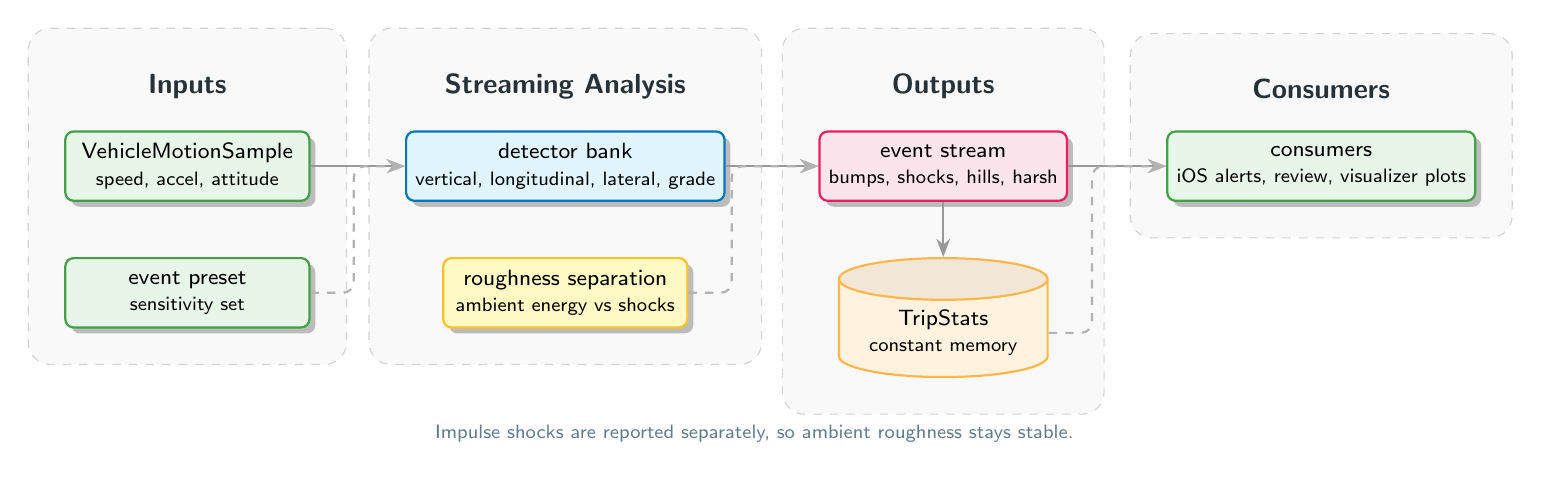
\begin{tikzpicture}[
    node distance=0.7cm and 1.35cm,
    font=\sffamily\footnotesize,
    >=Stealth,
    dataNode/.style={
        rectangle, rounded corners=3pt,
        draw=greenStroke, thick,
        fill=greenFill,
        minimum width=3.1cm, minimum height=0.88cm,
        align=center,
        drop shadow
    },
    opNode/.style={
        rectangle, rounded corners=3pt,
        draw=coreStroke, thick,
        fill=coreFill,
        minimum width=3.1cm, minimum height=0.88cm,
        align=center,
        drop shadow
    },
    procNode/.style={
        rectangle, rounded corners=3pt,
        draw=procStroke, thick,
        fill=procFill,
        minimum width=3.1cm, minimum height=0.88cm,
        align=center,
        drop shadow
    },
    optNode/.style={
        rectangle, rounded corners=3pt,
        draw=optStroke, thick,
        fill=optFill,
        minimum width=3.1cm, minimum height=0.88cm,
        align=center,
        drop shadow
    },
    memNode/.style={
        cylinder, cylinder uses custom fill,
        cylinder body fill=memFill, cylinder end fill=memFill!90!gray,
        shape border rotate=90,
        aspect=0.25,
        draw=memStroke, thick,
        minimum width=2.65cm, minimum height=1.0cm,
        align=center
    },
    group/.style={
        draw=gray!35, dashed, rounded corners=8pt,
        inner sep=13pt, fill=gray!5
    },
    title/.style={font=\sffamily\bfseries, text=textMain, align=center},
    note/.style={font=\sffamily\scriptsize, text=textMuted, align=center},
    flow/.style={->, thick, draw=gray!80, rounded corners=4pt},
    support/.style={->, thick, dashed, draw=gray!60, rounded corners=4pt}
]

% Layout plan: detector detail is summarized before routing to outputs, avoiding
% overlapping many-to-many event arrows.
\node[dataNode] (Sample) at (0, 0.85)
  {VehicleMotionSample\\\scriptsize speed, accel, attitude};
\node[dataNode, below=of Sample] (Preset) {event preset\\\scriptsize sensitivity set};
\node[title, above=0.28cm of Sample] (InputTitle) {Inputs};

\node[opNode] (Detectors) at (4.8, 0.85)
  {detector bank\\\scriptsize vertical, longitudinal, lateral, grade};
\node[procNode, below=of Detectors] (Roughness)
  {roughness separation\\\scriptsize ambient energy vs shocks};
\node[title, above=0.28cm of Detectors] (DetectorTitle) {Streaming Analysis};

\node[optNode] (Events) at (9.6, 0.85)
  {event stream\\\scriptsize bumps, shocks, hills, harsh};
\node[memNode, below=of Events] (Stats) {TripStats\\\scriptsize constant memory};
\node[title, above=0.28cm of Events] (OutputTitle) {Outputs};

\node[dataNode] (Consumers) at (14.4, 0.85)
  {consumers\\\scriptsize iOS alerts, review, visualizer plots};
\node[title, above=0.28cm of Consumers] (ConsumerTitle) {Consumers};

\node[note] (RoughnessNote) at (7.2, -2.55)
  {Impulse shocks are reported separately, so ambient roughness stays stable.};

\begin{scope}[on background layer]
  \node[group, fit=(InputTitle)(Sample)(Preset)] {};
  \node[group, fit=(DetectorTitle)(Detectors)(Roughness)] {};
  \node[group, fit=(OutputTitle)(Events)(Stats)] {};
  \node[group, fit=(ConsumerTitle)(Consumers)] {};
\end{scope}

\draw[flow] (Sample.east) -- (Detectors.west);
\draw[support] (Preset.east) -- ++(0.55,0) |- (Detectors.west);
\draw[flow] (Detectors.east) -- (Events.west);
\draw[flow] (Events.east) -- (Consumers.west);
\draw[flow] (Events.south) -- (Stats.north);
\draw[support] (Roughness.east) -- ++(0.55,0) |- (Events.west);
\draw[support] (Stats.east) -- ++(0.55,0) |- (Consumers.west);

\end{tikzpicture}
\end{document}
